\documentclass[12pt]{article}
\usepackage{graphicx}
\graphicspath{{Images/}}
\usepackage{textcomp} %for the copywrite symbol
%\linespread{1.6} %sets lines to 1.5 spacing.  1.6 would be double spaced
\usepackage[margin=1.0in]{geometry}
\usepackage[semicolon,round,sort&compress,sectionbib,numbers]{natbib}  
\usepackage{chapterbib}  
\usepackage{amsmath}
\usepackage{subcaption}
\usepackage{appendix} %for appendices
\usepackage{float}
\usepackage{listings}

\usepackage{hyperref} %make stuff clickable
\hypersetup{
	colorlinks,
	citecolor=black,
	filecolor=black,
	linkcolor=black,
	urlcolor=black
}


\usepackage{physics}  %for bras and kets!
\newcommand{\angstrom}{\mbox{\normalfont\AA }} %makes \angstrom do its thing!

\title{Lithium ELNES with WIEN2k}

\begin{document}
\maketitle


\section{Tools}	
Here's a list of software I use to run simulations.  I've put some installation instructions for linux as needed.  

\begin{itemize}
	\item Wien2k  -You either already have it installed somewhere, or should figure out how to do that before buying a license.  
	
	\item  VESTA: \url{http://jp-minerals.org/vesta/en/download.html}.  Download the .rpm file, install it with your package manager, eg. ``sudo apt-get vesta...rpm"
	
\end{itemize}
	
\section{Setup}	

We need a couple things to get started for ELNES simulations.  Foremost is a crystal structure.  You can either get this from the literature, XRD, or alternatively Materials Project: \url{https://materialsproject.org/}.  Download a cif (the primative cell typically) or enter the coordinates directly into the wien2k struct gen tool.  

Make a new Wien2k session: 
\begin{figure}[H]
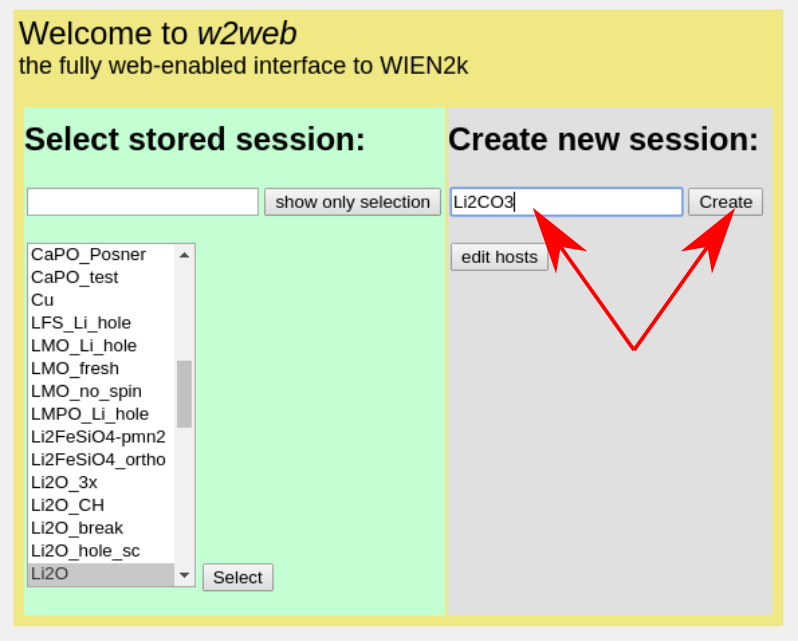
\includegraphics[scale=0.3]{./images/new_session.png}
\end{figure}

Create/change a working directory, and change the session information for parallel calculation.
	
	\begin{figure}[H]
		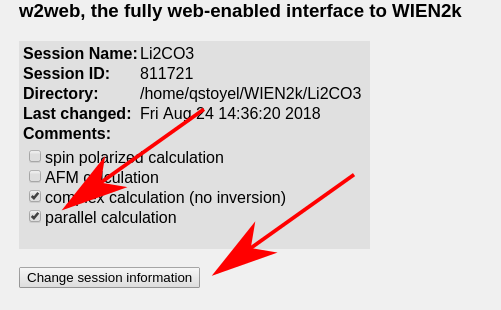
\includegraphics[scale=0.5]{./images/parallel.png}
	\end{figure}
	
You will also need to make a ``.machines" file which you can either steal from one of my directories, look in the user guide and make your own, cut and paste the one from below, or wait for w2web to automatically generate one at some point after it inevitably crashes on something.
Sample .machines file: 

\begin{lstlisting}
#=======================================
#This is a valid .machines file
#
granularity:1
1:localhost #as many of these lines as you want cpu cores running
1:localhost
1:localhost
1:localhost
1:localhost
1:localhost

\end{lstlisting}

Next, go make a struct file, with struct gen, either by importing the cif, or entering the positions manually.  Use VESTA (drag n' drop the .struct file) to make sure that the structure is what you'd expect. 
In our Li2CO3 case this looks like: 

	\begin{figure}[H]
	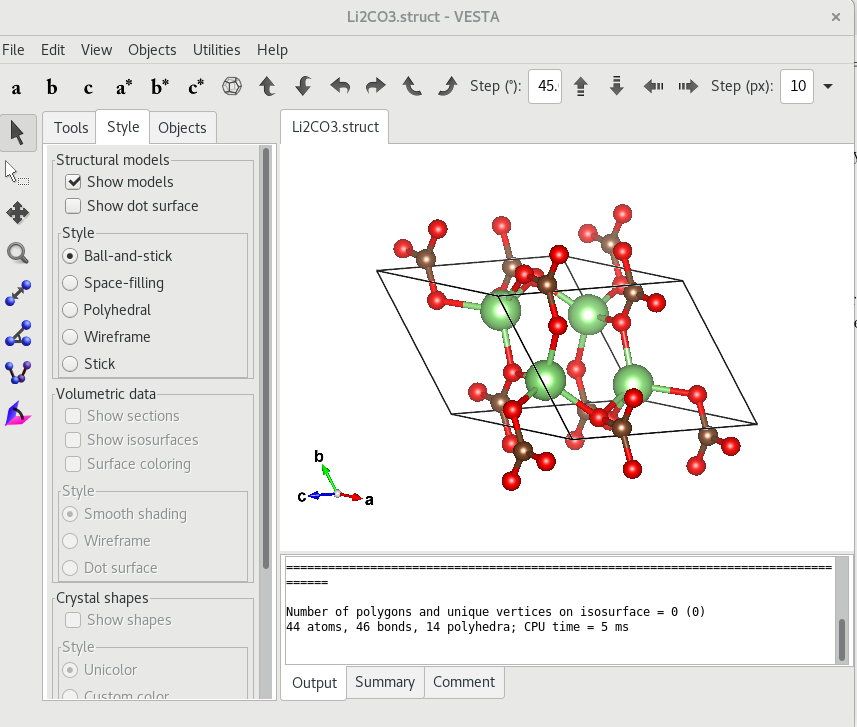
\includegraphics[scale=0.4]{./images/Li2CO3_struct.png}
\end{figure}


Now we need to initialize the case.  You can do this in w2web, but we are going to get our hands dirty anyways, so I like to use the command line for this and see what's actually going on.  Run ``init\_lapw" in the case directory.

\begin{itemize}
	\item \textbf{setrmt}. Sets the muffin tin size on the atoms.  Reduce the sphere size by 0\% using either old or new scheme and accept, it doesn't matter much as we are going to change this all later.
	\item  \textbf{nn}.  Checks for overlapping muffin tins. Enter ``2.0", close the first file and use the new NN file if it suggests it, run nn with 2.0 again, look at how much ``wiggle room" you have on the spheres, see pic. 
	
	\begin{figure}[H]
		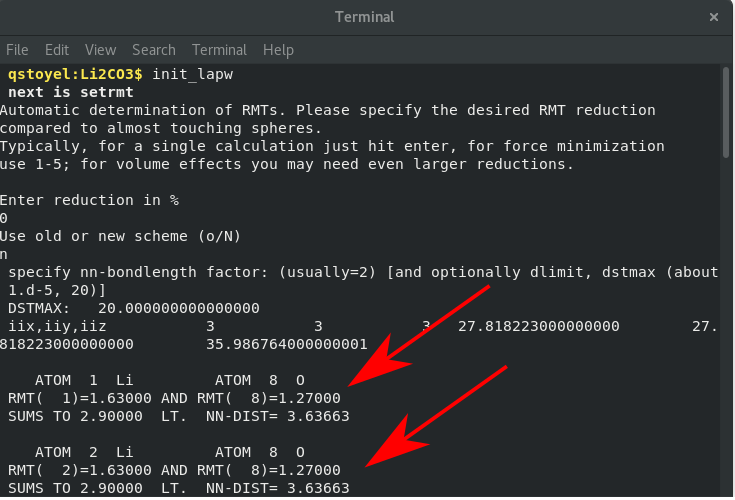
\includegraphics[scale=0.4]{./images/init_lapw2.png}
	\end{figure}
	
	\item \textbf{sgroup}. Verifies the space group.  Again, accept any changes the program makes, these steps are all about reducing the cell symmetries to what they should be. Again, the files can be largely  ignored at this point, with the exception of indication of a Bravais lattice change, in which case just take the new struct file. If so, nn and sgroup will run again with ``nice" results.  
	\item  \textbf{symmery}. Generates all the symmetry operations. Run it and continue (enter ``c")
	\item  \textbf{lstart}. Set spin state, pick your XC kernel, define cutoff between core and valence states.  Accept default spins, unless you have a transition metal, and  and GGA PBE as you XC potential. Picking the energy is the most important part of this first run init\_lapw, we want to try to get the Li 1s states to be treated as core states.  They typically have energies of $\sim$-3.5Ry, so try with that first, and look in case.outputst (the file that pops up), for the following lines for the lithium atom and look at the 1S states:  
	
	\begin{lstlisting}
          E-up(Ry)      E-dn(Ry)   Occupancy   q/sphere  core-state
1S      -3.801947     -3.785288  1.00  1.00    0.9859  T
1S      -3.801947     -3.785288  1.00  1.00    0.9859  T
2S      -0.236699     -0.003313  1.00  0.00    0.0468  F
2S      -0.236699     -0.003313  1.00  0.00    0.0468  F
	\end{lstlisting}
	
	These indicate the core states (T/F), their energy levels (in this case $\sim$ -3.8eV) and how much the electrons in these states live in the muffin tins (0.9859).  As this is less than 1, it means a lot of 1S lithium electron is leaking out of the muffin tins, which is why there should now be all kinds of warnings popping up.  So go ahead and ``ctrl-c" out of init\_lapw.
	
\end{itemize}  

To fix the leakage problem, we need to make the Lithium muffin tins bigger. We want to make them just big enough to hold all of the 1S electrons, without making them too different from the other muffin tins, as the larger this difference, the harder things get to calculate/converge.  In this case we try Li=1.8,  C=1.2, O=1.22 and try init\_lapw again.  

\begin{itemize}
	\item \textbf{setrmt}: Setrmt will try to reset the muffin tins to the defaults, make sure to discard these (enter d)
	\item \textbf{nn} Make sure you don't get errors, and that everything is as tight as it can be, in this case the Oxygen-carbon spacing is the limiting factor.  
	\item \textbf{sgroup} Should run fine.
	\item  \textbf{symmery} Should run fine. 
	\item \textbf{lstart} Rewrite the old file, note increase in electron containment for Lithium (0.9922) in case.outputst.  Go back and loop through increasing the muffin tins a little more (1.85,1.9,2.0) and checking the containment until it gets above 0.995 and the warnings stop.  
	\item \textbf{kgen} Set the RkMax value in case.in1\_st:		
	\begin{figure}[H]
		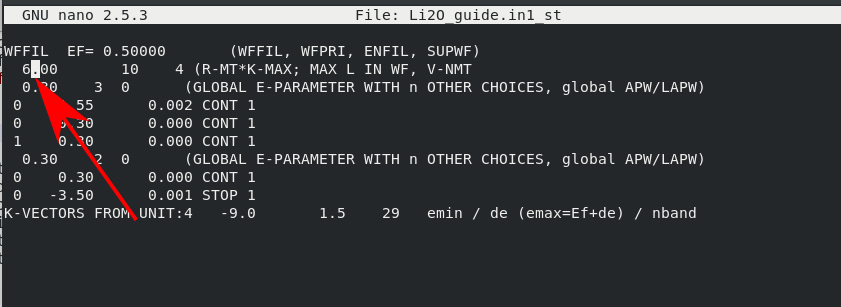
\includegraphics[scale=0.4]{./images/init_lapw3.png}
	\end{figure}
	and then pick a k\_point number.  Both of these values should be taken for fast convergence, in this case I chose RkMax=7.0, and 16 k points.
	\item \textbf{Dstart}: make sure to pick non spin polarized, unless you have reason to believe otherwise (is there a transition metal in your sample?)
\end{itemize}

Assuming tere were no warnings in the final run through init\_lapw, we can now start convergence.

\section{Convergence}
Ideally, you want to converge everything regarding your simulation.  Typically this is cell parameters, k points and Rkmax.  The first step is to just make sure the calculation converges, running it with a small RKmax and few kpoints and making sure it finishes.  

\subsection{Cell parameters:}
This process works best from W2Web, as described in the tutorials.  You might need to make your muffin tins smaller to avoid nn errors.  You can this with the muffin tins we picked out above, or just use the ones \textbf{setrmt} suggests and reduce them by 5-10\%.  As you need run a number (5-11+) of calculations, you want to use low k points and RKMax values, for Li2CO3, I used 64 kpoints and an RKmax of 7 initially.   In the x ``optimize" tab, choose what you want to optimize, the first option (volume) is typically sufficient, unless you have suspicions otherwise.  Enter a range of values of test volumes, see picture:

\begin{figure}[H]

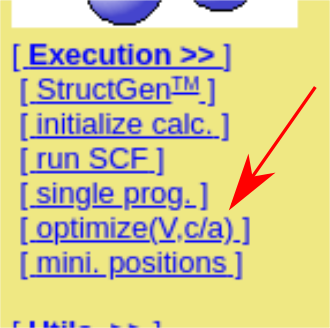
\includegraphics[scale=0.3]{./images/vol_opt_menu.png}
~
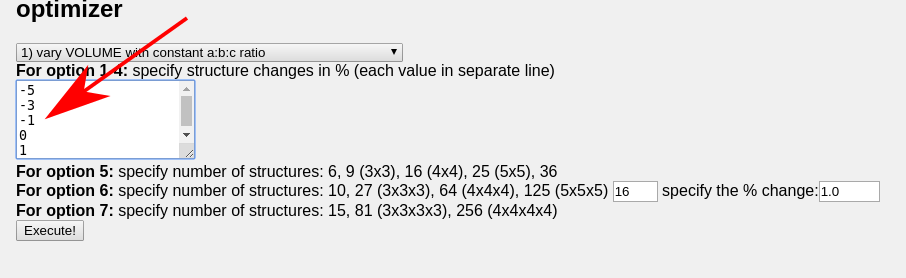
\includegraphics[scale=0.3]{./images/vol_opt.png}



\end{figure}


Also make sure to edit ``optimize.job" to enable parallization by moving the ``\#" to after the ``-p" in the run\_lapw line: 

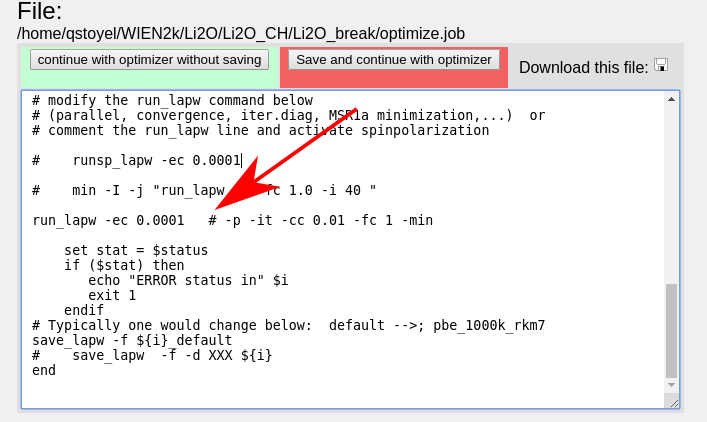
\includegraphics[scale=0.4]{./images/vol_opt2.png}

You can then ``run optimize.job" from w2web.



\section{Common Errors Thrown by Code}

\subsection{GMax Value less than Gmin}

Occurs in \textbf{dstart}, fix is to bump up the Gmax value in case.in2 from 12.00 to 14.00 or 16.00.

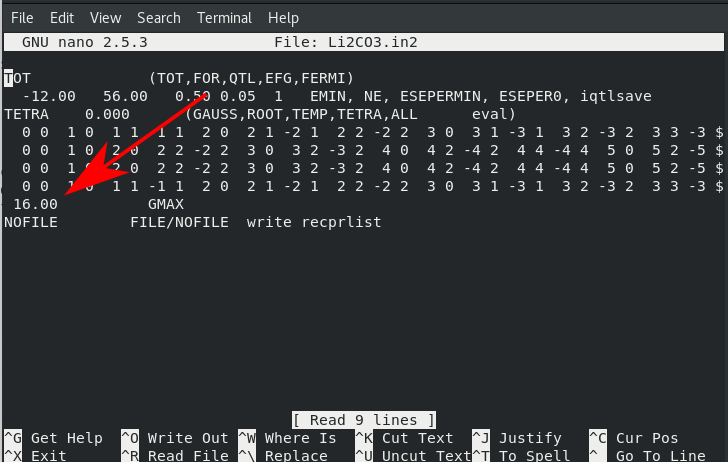
\includegraphics[scale=0.5]{./images/gmax_err.png}


\subsection{K point and RKMax convergence}

To converge these parameters, again start with very low values and then increase them, checking the total energy to determine when they are converged.  I like to start with k points and then move on to RKMax.  To bump up the values, you want to either rerun ``x kgen" and enter a larger k point value, or edit case.in1 and case.in1\_st, and increase the RKMax


\begin{itemize}
	\item \textbf{setrmt}
	\item \textbf{nn}
	\item \textbf{sgroup}
	\item  \textbf{symmery}
	\item \textbf{lstart}
	
\end{itemize}


\end{document}